\documentclass[10pt]{beamer}

\setbeamersize{text margin left=0.5cm, text margin right=0.5cm}

\usepackage{alltt}%
%\usetheme{Boadilla}
\usetheme[progressbar = foot, background=light]{metropolis} 
%\useoutertheme{split}

%\usecolortheme{beaver}

%\usepackage{listings}
\makeatletter
\def\maxwidth{ %
  \ifdim\Gin@nat@width>\linewidth
    \linewidth
  \else
    \Gin@nat@width
  \fi
}
\makeatother

\definecolor{fgcolor}{rgb}{0.345, 0.345, 0.345}
\newcommand{\hlnum}[1]{\textcolor[rgb]{0.686,0.059,0.569}{#1}}%
\newcommand{\hlstr}[1]{\textcolor[rgb]{0.192,0.494,0.8}{#1}}%
\newcommand{\hlcom}[1]{\textcolor[rgb]{0.678,0.584,0.686}{\textit{#1}}}%
\newcommand{\hlopt}[1]{\textcolor[rgb]{0,0,0}{#1}}%
\newcommand{\hlstd}[1]{\textcolor[rgb]{0.345,0.345,0.345}{#1}}%
\newcommand{\hlkwa}[1]{\textcolor[rgb]{0.161,0.373,0.58}{\textbf{#1}}}%
\newcommand{\hlkwb}[1]{\textcolor[rgb]{0.69,0.353,0.396}{#1}}%
\newcommand{\hlkwc}[1]{\textcolor[rgb]{0.333,0.667,0.333}{#1}}%
\newcommand{\hlkwd}[1]{\textcolor[rgb]{0.737,0.353,0.396}{\textbf{#1}}}%
\let\hlipl\hlkwb

\usepackage{framed}
\makeatletter
\newenvironment{kframe}{%
 \def\at@end@of@kframe{}%
 \ifinner\ifhmode%
  \def\at@end@of@kframe{\end{minipage}}%
  \begin{minipage}{\columnwidth}%
 \fi\fi%
 \def\FrameCommand##1{\hskip\@totalleftmargin \hskip-\fboxsep
 \colorbox{shadecolor}{##1}\hskip-\fboxsep
     % There is no \\@totalrightmargin, so:
     \hskip-\linewidth \hskip-\@totalleftmargin \hskip\columnwidth}%
 \MakeFramed {\advance\hsize-\width
   \@totalleftmargin\z@ \linewidth\hsize
   \@setminipage}}%
 {\par\unskip\endMakeFramed%
 \at@end@of@kframe}
\makeatother

\definecolor{shadecolor}{rgb}{.97, .97, .97}
\definecolor{messagecolor}{rgb}{0, 0, 0}
\definecolor{warningcolor}{rgb}{1, 0, 1}
\definecolor{errorcolor}{rgb}{1, 0, 0}
\newenvironment{knitrout}{}{} % an empty environment to be redefined in TeX
    
\usepackage[utf8]{inputenc}
\usepackage{default}

\usepackage{xcolor}%for color mixing

\usepackage{amsmath}%
\usepackage{amsfonts}%
\usepackage{amssymb}%
\usepackage{graphicx}

\usepackage{tikz}


\setbeamertemplate{itemize/enumerate body begin}{\small}

%%%%%%%%%%%%%%%%%%%%%%%%%%%%%%%%%%%%%%%%%%%%%%%%%%%%%%%%%%%%%%%%%%%%%%%%%%%%%%%%%%

%%%%%%%%%%%%%%%%%%%%%%%%%%%%%%%%%%%%%%%%%%%%%%%%%%%%%%%%%%%%%%%%%%%%%%%%%%%%%%%%%%

\title{Introduction to Experimental Design}
\subtitle{Chapter 2}
\author{Timoth\'ee Bonnet and Terry Neeman}
\date{\today}

\begin{document}

%\lstset{language=R}%code

\AtBeginSection[]
{
  \begin{frame}<beamer>
    \frametitle{}
    \tableofcontents[currentsection,sectionstyle=show/show,subsectionstyle=show/shaded/hide]% down vote\tableofcontents[currentsection,currentsubsection,hideothersubsections,sectionstyle=show/hide,subsectionstyle=show/shaded/hide] 
  \end{frame}
}


\begin{frame}{}
\maketitle

\end{frame}
%%%%%%%%%%%%%%%%%%%%%%%

\begin{frame}{``Experimental design'' ?}
 
 \begin{exampleblock}{Relevant for}
  \begin{itemize}[<+->]
   \item Designing lab / field manipulative experiments
      \begin{itemize}
       \item Isolate the process of interest
       \item Avoid problems with confounding variables
      \end{itemize}
   \item Collecting any kind of data 
   \begin{itemize}
       \item Isolate the process of interest
       \item Avoid problems with confounding variables
      \end{itemize}
   \item Analyzing any kind of data (even if you do not design the experiment or data collection)
      \begin{itemize}
       \item Understand data structure
       \item Fit models appropriate for data structure and experimental design
       \item Detect confounding and statistically correct for it if possible
      \end{itemize}

  \end{itemize}  
 \end{exampleblock}

 
\end{frame}
%%%%%%%%%%%%

\begin{frame}{KEY PRINCIPLES in Experimental Design}

\begin{alertblock}{}
 \begin{itemize}
  \item Controls
  \item Replication
  \item Blocking
  \item Randomisation
  \item Blinding
 \end{itemize}

\end{alertblock}

\end{frame}
%%%%%%%%%%%%%%%%%%%%%%%


\begin{frame}{KEY PRINCIPLES in Experimental Design}

\begin{alertblock}{}
 \begin{itemize}
  \item {\color{red}{Controls}}
    \begin{itemize}
     \item Direct comparison with a known standard or no treatment.
      \item Tested under identical conditions to experimental treatment.
    \end{itemize}
  \item Replication
  \item Blocking
  \item Randomisation
  \item Blinding
 \end{itemize}

\end{alertblock}

\end{frame}
%%%%%%%%%%%%%%%%%%%%%%%


\begin{frame}{KEY PRINCIPLES in Experimental Design}

\begin{alertblock}{}
 \begin{itemize}
  \item Controls
  \item {\color{red}{Replication}} repeating experiment on different samples to: 
    \begin{enumerate}
      \item Increase precision of treatment effect
      \item Make result more generalisable
    \end{enumerate}
  \item Blocking
  \item Randomisation
  \item Blinding
 \end{itemize}

\end{alertblock}

\end{frame}
%%%%%%%%%%%%%%%%%%%%%%%


\begin{frame}{KEY PRINCIPLES in Experimental Design}

\begin{alertblock}{}
 \begin{itemize}
  \item Controls
  \item Replication
  \item {\color{red}{Blocking}}
    \begin{itemize}
     \item Grouping together similar experimental units
     \item Comparing treatments within homogeneous groups
    \end{itemize}
  \item Randomisation
  \item Blinding
 \end{itemize}

\end{alertblock}

\end{frame}
%%%%%%%%%%%%%%%%%%%%%%%


\begin{frame}{KEY PRINCIPLES in Experimental Design}

\begin{alertblock}{}
 \begin{itemize}
  \item Controls
  \item Replication
  \item Blocking
  \item {\color{red}{Randomisation}}
    \begin{itemize}
     \item probabilistic process of assigning treatment
     \item randomising order of testing
    \end{itemize}
  \item Blinding
 \end{itemize}

\end{alertblock}

\end{frame}
%%%%%%%%%%%%%%%%%%%%%%%


\begin{frame}{KEY PRINCIPLES in Experimental Design}

\begin{alertblock}{}
 \begin{itemize}
  \item Controls
  \item Replication
  \item Blocking
  \item Randomisation
  \item {\color{red}{Blinding}} Masking treatment assignment
    \begin{itemize}
     \item Allocation blinded
     \item Evaluator blinded
    \end{itemize}
 \end{itemize}

\end{alertblock}

\end{frame}
%%%%%%%%%%%%%%%%%%%%%%%

\begin{frame}{Example: Converging on an experimental design using these key principles}
 \begin{columns}
  \begin{column}{0.5\textwidth}
  \textbf{Research context:}
    \begin{itemize}
     \item What are the essential elements of chloroquine transporters in malaria parasites?
     \item Methods: oocyte system, radiotracer assay
     \item Treatments: 5 mutant transporters plus wild type
    \end{itemize}
  \end{column}
  \begin{column}{0.5\textwidth}
    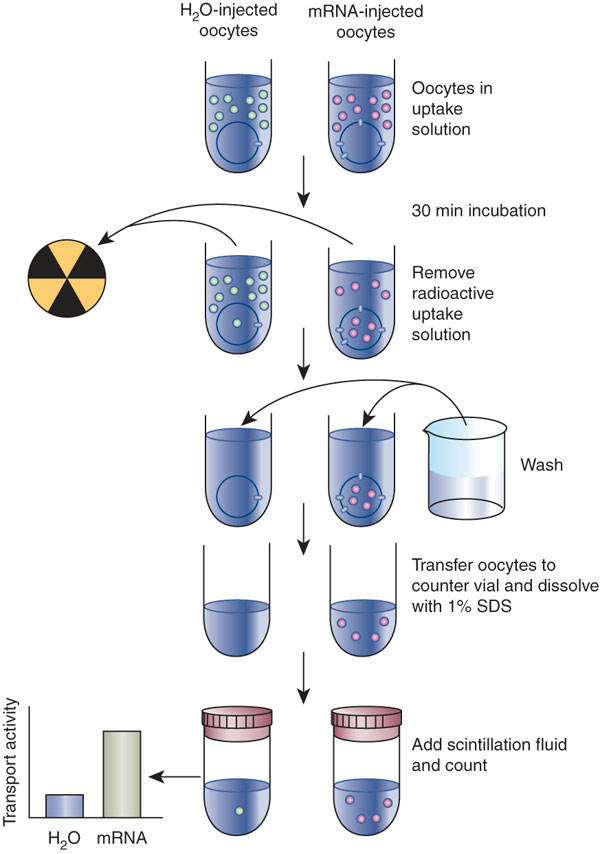
\includegraphics[height=0.8\textheight]{Figures/expdesign}
  \end{column}

 \end{columns}

\end{frame}
%%%%%%%%%%%%%%

\begin{frame}{Experimental design: chloroquine transporters}
 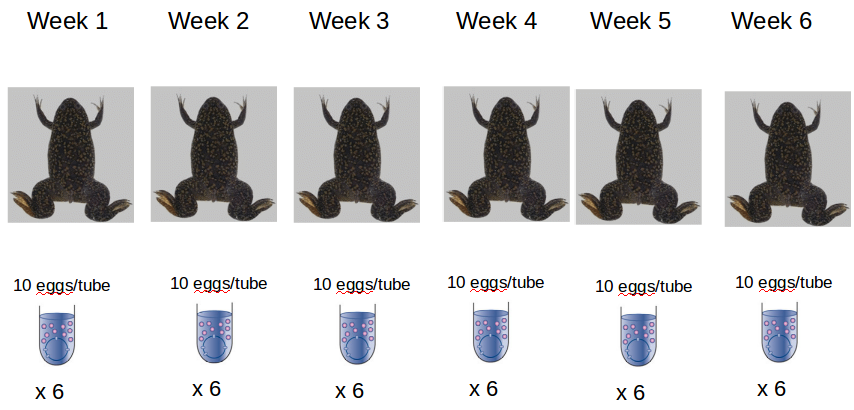
\includegraphics[width=\textwidth]{Figures/expdes1}
\end{frame}
%%%%%%%%%%%%


\begin{frame}{Experimental design: chloroquine transporters}
 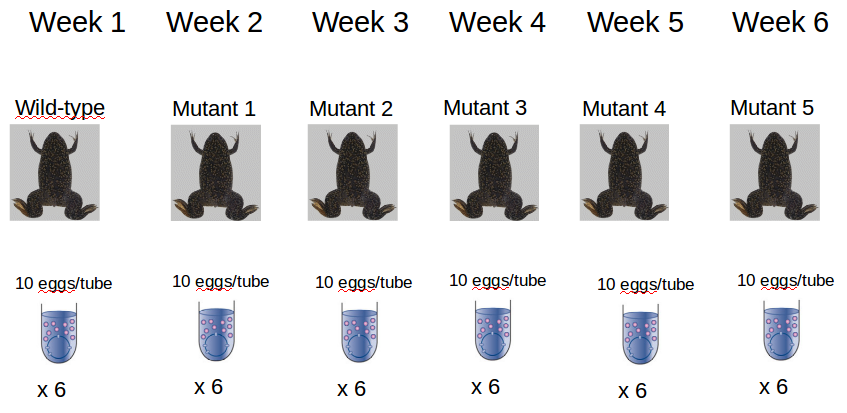
\includegraphics[width=\textwidth]{Figures/expdes2}
 \pause
 
 \emph{\textbf{What is wrong with this design?}}
\end{frame}
%%%%%%%%%%%%


\begin{frame}{What is wrong with this design?}
 \begin{alertblock}{}
 \begin{itemize}
  \item CONTROLS: not tested under identical conditions
  \item REPLICATION: only pseudo-replication
  \item BLOCKING: none
  \item RANDOMISATION: NA
 \end{itemize}
 \end{alertblock}
 
 \pause
 
 Experiment is useless

\end{frame}
%%%%%%%%%%%%
\begin{frame}{How about this design}
 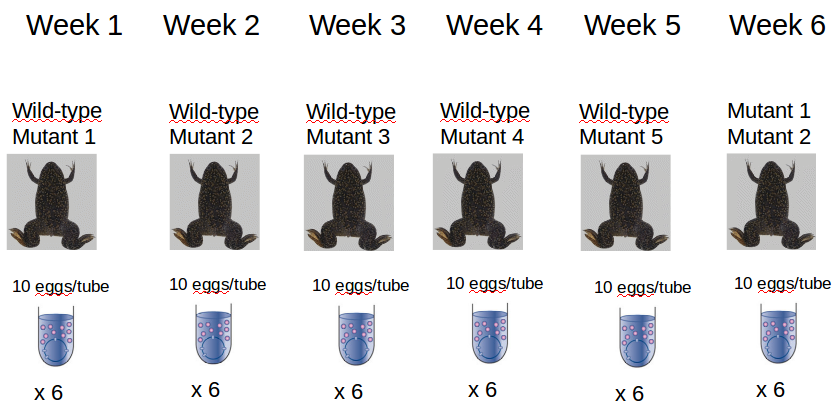
\includegraphics[width=\textwidth]{Figures/expdes3}
 \pause
 
 \emph{\textbf{What is wrong with this design?}}
\end{frame}
%%%%%%%%%%%%


\begin{frame}{What is wrong with this design?}
 \begin{alertblock}{}
 \begin{itemize}
  \item CONTROLS: just okay, can compare control to each mutant; not between mutants
  \item BLOCKING: frog=block, not all treatments for each block
  \item REPLICATION: no replication of any comparison
  \item RANDOMISATION: could randomise tubes within day
 \end{itemize}
 Also, half the eggs were used for control treatment: is this the most efficient use of resources?
 \end{alertblock}
 
\end{frame}
%%%%%%%%%%%%

%%%%%%%%%%%%
\begin{frame}{How about this design}
 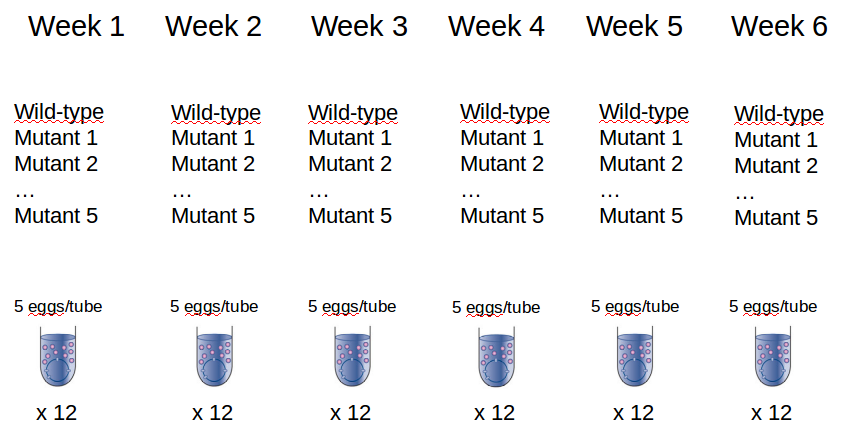
\includegraphics[width=\textwidth]{Figures/expdes4}
\end{frame}
%%%%%%%%%%%%


\begin{frame}{A good design}
 \begin{alertblock}{}
 \begin{itemize}
  \item CONTROLS: yes, can compare control to each mutant, and each mutant to every other
  \item BLOCKING: frog=block, complete randomised design
  \item REPLICATION: each block is a replicate
  \item RANDOMISATION: could randomise tubes within day
 \end{itemize}
 \end{alertblock}
 
\end{frame}
%%%%%%%%%%%%

\begin{frame}{Example 2}
 \textbf{How can the design of this experiment (control + 2 treatments) be improved?}
 
 \centering
 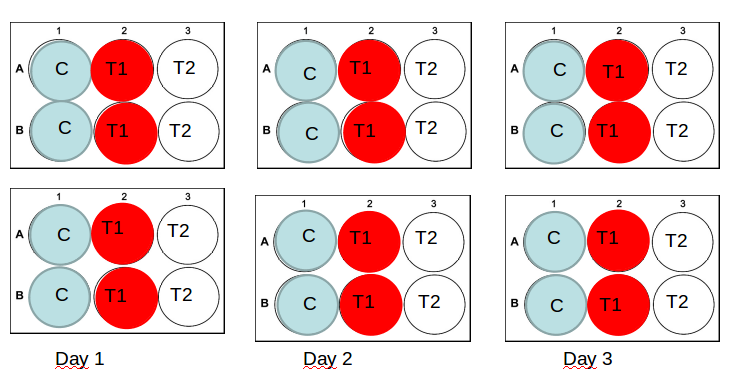
\includegraphics[width=0.9\textwidth]{Figures/expdesb}
\end{frame}
%%%%%%%%%%%%

\begin{frame}{Example 3}
 \textbf{What are the possible sources of variation on a plate for a PCR / cell viability plate / plant experiment}
 
 \centering
 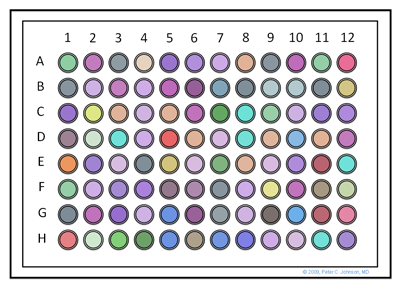
\includegraphics[width=0.8\textwidth]{Figures/expdesc}
\end{frame}
%%%%%%%%%%%%

\begin{frame}{Example 4}
Cochrane et al. Oikos (2014)
\begin{block}{Research context}
\begin{itemize}
  \item How is seedling emergence (in Banksia) influenced by temperature and moisture?
  \item Set up: 12 shelters, 2 garden beds per shelter, 24 pots per bed.
  \item Experimental factors: 
    \begin{itemize}
      \item Temperature (2 levels)
      \item Water (3 levels)
      \item Species (4 levels) 
      \item Populations (6 per species = 24)
     \end{itemize}
\end{itemize}
\end{block}

\end{frame}
%%%%%%%%%%%%

\begin{frame}{Example 4}
\textbf{How to distribute treatments across 12 shelters?}
  \centering
  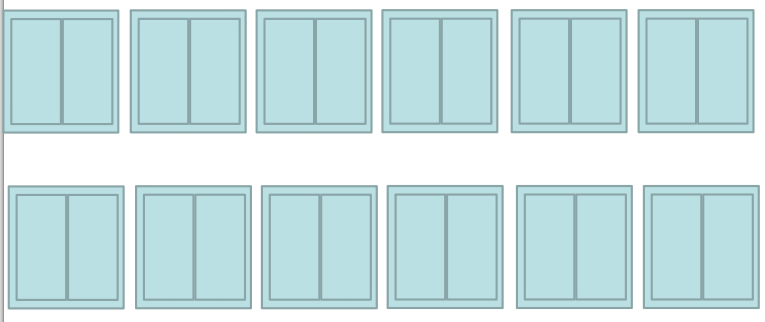
\includegraphics[width=\textwidth]{Figures/shelters}
\end{frame}
%%%%%%%%%%%


\begin{frame}{Example 4}
\textbf{How to distribute treatments across 12 shelters?\\}
 Hot temperature in {\color{orange}{orange}}, cold in {\color{blue!50!green}{turquoise}}\\
  \centering
  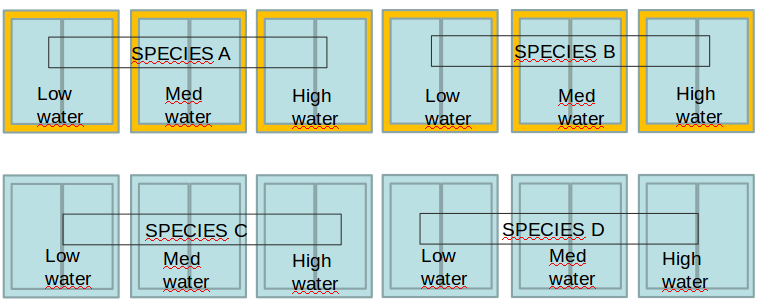
\includegraphics[width=\textwidth]{Figures/shelters2}
  
  \pause
  \vspace{0.1cm}
  \textbf{What’s wrong with this design?}
\end{frame}
%%%%%%%%%%%



\begin{frame}{Example 4}
\textbf{How to distribute treatments across 12 shelters?\\ How about this design?}
\begin{itemize}
 \item Hot temperature in top shelters, cold in bottom shelters
 \item repeat A/B/C/D in each shelter
\end{itemize}

  \centering
  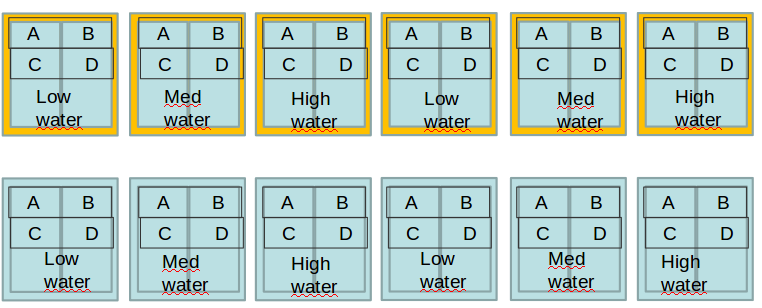
\includegraphics[width=\textwidth]{Figures/shelters3}
\end{frame}
%%%%%%%%%%%


\begin{frame}{Example 4}
\textbf{How to distribute treatments across 12 shelters?\\ How about this design?}
\begin{itemize}
 \item Hot and cold temperatures by bed (randomized left/right)
 \item repeat A/B/C/D in each shelter
\end{itemize}
  \centering
  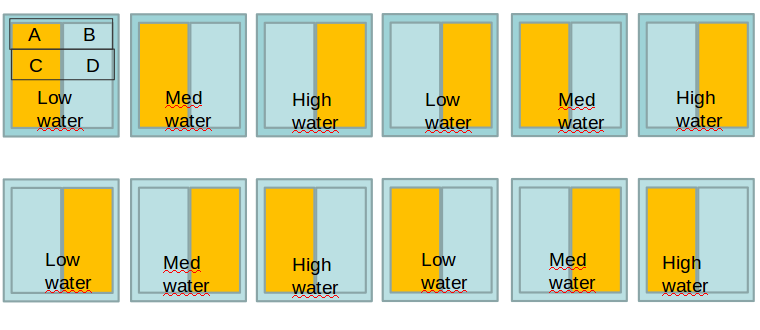
\includegraphics[width=\textwidth]{Figures/shelters4}
\end{frame}
%%%%%%%%%%%

\begin{frame}{Example 4}
\textbf{How to distribute treatments across 12 shelters?\\ How about this design?}
\begin{itemize}
 \item Hot and cold temperatures by bed (randomized left/right)
 \item repeat A/B/C/D in each row (randomized within row)
 \item Humidity in each bed (randomized among columns)
\end{itemize}
  \centering
  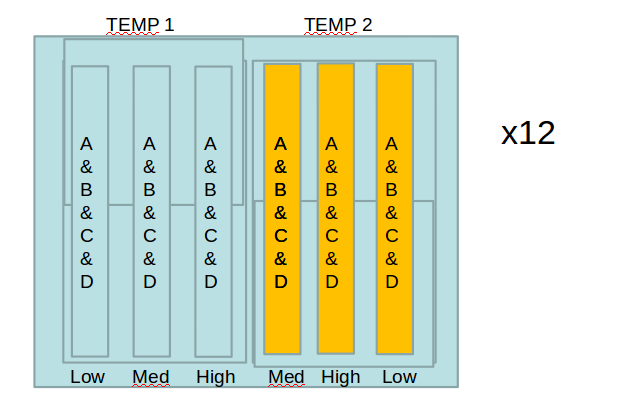
\includegraphics[width=0.6\textwidth]{Figures/shelters5}
\end{frame}
%%%%%%%%%%%


\begin{frame}{Reading}

 \begin{itemize}
  \item Chapter 3, Statistical methods in biology, Welham et al
  \item Kilkenny et al ARRIVE guidelines
  \item Ten Simple Rules for Effective Statistical Practice
 \end{itemize}

\end{frame}
%%%%%%%%%%%

\end{document}
